\documentclass{standalone}
\usepackage{tikz}
\usetikzlibrary{patterns, positioning}


\begin{document}
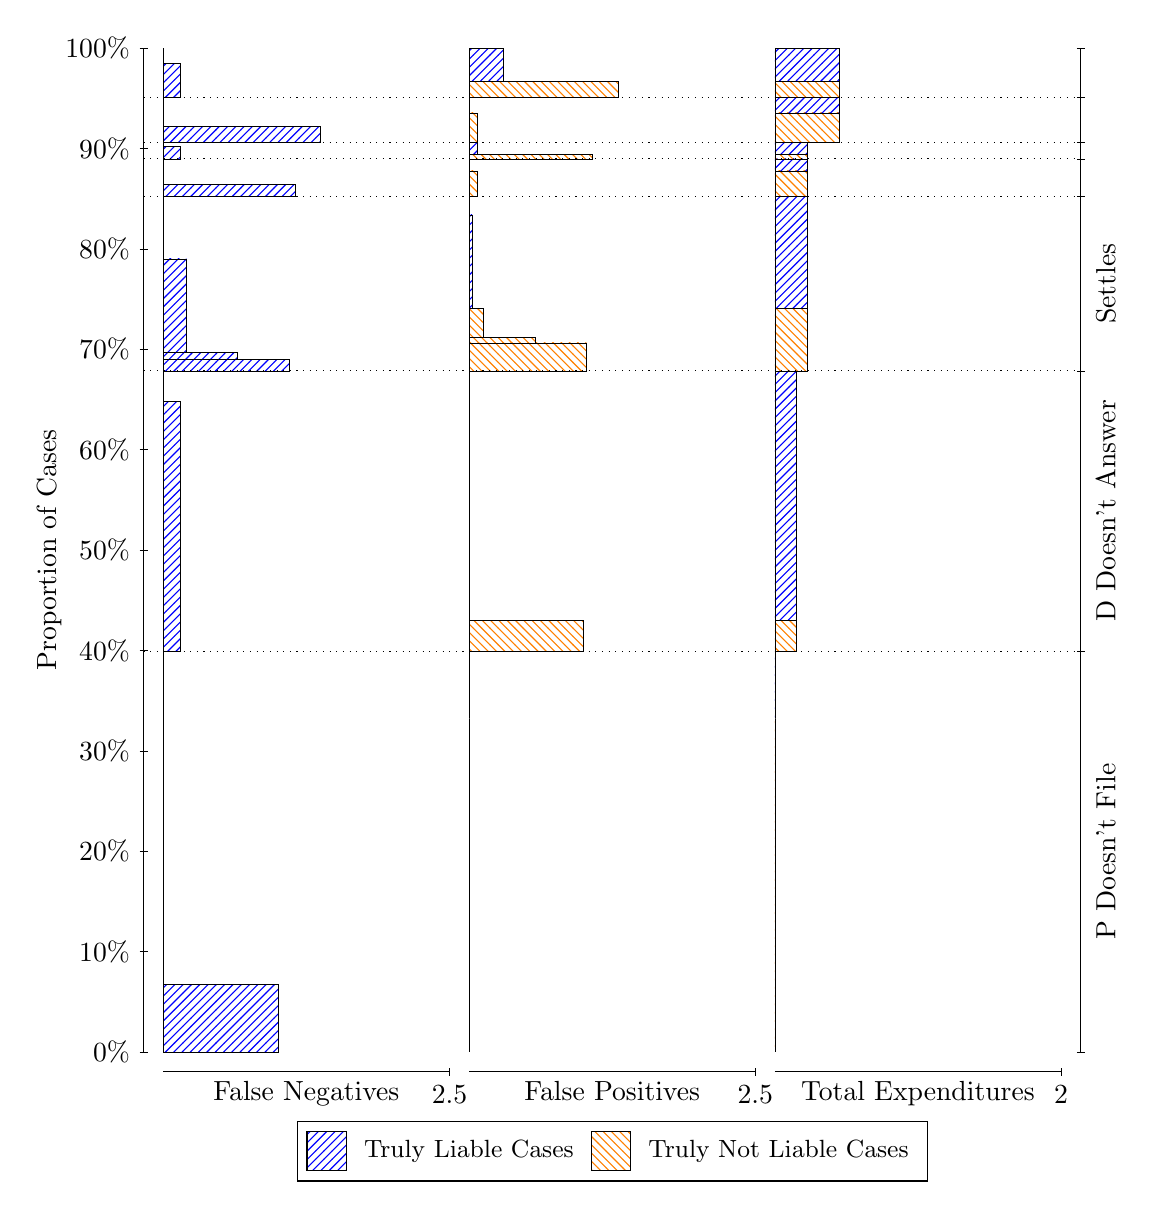
\begin{tikzpicture}
\draw[black, very thin] (1.5,1.75) -- (1.5,14.5);
\node[rotate=90, text=black, anchor=center] at (0.3, 8.125) {Proportion of Cases};
\draw[black, very thin] (1.45,1.75) -- (1.55,1.75);
\node[text=black, anchor=east] at (1.45, 1.75) {0\%};
\draw[black, very thin] (1.45,3.025) -- (1.55,3.025);
\node[text=black, anchor=east] at (1.45, 3.025) {10\%};
\draw[black, very thin] (1.45,4.3) -- (1.55,4.3);
\node[text=black, anchor=east] at (1.45, 4.3) {20\%};
\draw[black, very thin] (1.45,5.575) -- (1.55,5.575);
\node[text=black, anchor=east] at (1.45, 5.575) {30\%};
\draw[black, very thin] (1.45,6.85) -- (1.55,6.85);
\node[text=black, anchor=east] at (1.45, 6.85) {40\%};
\draw[black, very thin] (1.45,8.125) -- (1.55,8.125);
\node[text=black, anchor=east] at (1.45, 8.125) {50\%};
\draw[black, very thin] (1.45,9.4) -- (1.55,9.4);
\node[text=black, anchor=east] at (1.45, 9.4) {60\%};
\draw[black, very thin] (1.45,10.675) -- (1.55,10.675);
\node[text=black, anchor=east] at (1.45, 10.675) {70\%};
\draw[black, very thin] (1.45,11.95) -- (1.55,11.95);
\node[text=black, anchor=east] at (1.45, 11.95) {80\%};
\draw[black, very thin] (1.45,13.225) -- (1.55,13.225);
\node[text=black, anchor=east] at (1.45, 13.225) {90\%};
\draw[black, very thin] (1.45,14.5) -- (1.55,14.5);
\node[text=black, anchor=east] at (1.45, 14.5) {100\%};

\draw[black, very thin] (13.4,1.75) -- (13.4,14.5);
\draw[black, very thin] (13.35,1.75) -- (13.45,1.75);
\node[anchor=west] at (13.35, 1.75) {};
\draw[black, very thin] (13.35,6.8406) -- (13.45,6.8406);
\node[anchor=west] at (13.35, 6.8406) {};
\draw[black, very thin] (13.35,10.401) -- (13.45,10.401);
\node[anchor=west] at (13.35, 10.401) {};
\draw[black, very thin] (13.35,12.615) -- (13.45,12.615);
\node[anchor=west] at (13.35, 12.615) {};
\draw[black, very thin] (13.35,13.093) -- (13.45,13.093);
\node[anchor=west] at (13.35, 13.093) {};
\draw[black, very thin] (13.35,13.305) -- (13.45,13.305);
\node[anchor=west] at (13.35, 13.305) {};
\draw[black, very thin] (13.35,13.877) -- (13.45,13.877);
\node[anchor=west] at (13.35, 13.877) {};
\draw[black, very thin] (13.35,14.5) -- (13.45,14.5);
\node[anchor=west] at (13.35, 14.5) {};

\draw[black, very thin, pattern color=blue, pattern=north east lines] (1.75,1.75) rectangle (3.2033,2.6054);
\draw[black, very thin, pattern color=orange, pattern=north west lines] (1.75,2.6054) rectangle (1.75,6.8406);
\draw[black, very thin, pattern color=blue, pattern=north east lines] (1.75,6.8406) rectangle (1.968,10.009);
\draw[black, very thin, pattern color=orange, pattern=north west lines] (1.75,10.009) rectangle (1.75,10.401);
\draw[black, very thin, pattern color=blue, pattern=north east lines] (1.75,10.401) rectangle (3.3487,10.544);
\draw[black, very thin, pattern color=blue, pattern=north east lines] (1.75,10.544) rectangle (2.6947,10.634);
\draw[black, very thin, pattern color=blue, pattern=north east lines] (1.75,10.634) rectangle (2.0407,11.822);
\draw[black, very thin, pattern color=orange, pattern=north west lines] (1.75,11.822) rectangle (1.75,12.615);
\draw[black, very thin, pattern color=blue, pattern=north east lines] (1.75,12.615) rectangle (3.4213,12.767);
\draw[black, very thin, pattern color=orange, pattern=north west lines] (1.75,12.767) rectangle (1.75,13.093);
\draw[black, very thin, pattern color=blue, pattern=north east lines] (1.75,13.093) rectangle (1.968,13.248);
\draw[black, very thin, pattern color=orange, pattern=north west lines] (1.75,13.248) rectangle (1.75,13.305);
\draw[black, very thin, pattern color=blue, pattern=north east lines] (1.75,13.305) rectangle (3.7483,13.506);
\draw[black, very thin, pattern color=orange, pattern=north west lines] (1.75,13.506) rectangle (1.75,13.877);
\draw[black, very thin, pattern color=blue, pattern=north east lines] (1.75,13.877) rectangle (1.968,14.3);
\draw[black, very thin, pattern color=orange, pattern=north west lines] (1.75,14.3) rectangle (1.75,14.5);
\draw[black, very thin, pattern color=orange, pattern=north west lines] (5.6333,1.75) rectangle (5.6333,5.9852);
\draw[black, very thin, pattern color=blue, pattern=north east lines] (5.6333,5.9852) rectangle (5.6333,6.8406);
\draw[black, very thin, pattern color=orange, pattern=north west lines] (5.6333,6.8406) rectangle (7.0867,7.2328);
\draw[black, very thin, pattern color=blue, pattern=north east lines] (5.6333,7.2328) rectangle (5.6333,10.401);
\draw[black, very thin, pattern color=orange, pattern=north west lines] (5.6333,10.401) rectangle (7.123,10.754);
\draw[black, very thin, pattern color=orange, pattern=north west lines] (5.6333,10.754) rectangle (6.469,10.827);
\draw[black, very thin, pattern color=orange, pattern=north west lines] (5.6333,10.827) rectangle (5.815,11.195);
\draw[black, very thin, pattern color=blue, pattern=north east lines] (5.6333,11.195) rectangle (5.6697,12.382);
\draw[black, very thin, pattern color=blue, pattern=north east lines] (5.6333,12.382) rectangle (5.6333,12.615);
\draw[black, very thin, pattern color=orange, pattern=north west lines] (5.6333,12.615) rectangle (5.7423,12.941);
\draw[black, very thin, pattern color=blue, pattern=north east lines] (5.6333,12.941) rectangle (5.6333,13.093);
\draw[black, very thin, pattern color=orange, pattern=north west lines] (5.6333,13.093) rectangle (7.1957,13.15);
\draw[black, very thin, pattern color=blue, pattern=north east lines] (5.6333,13.15) rectangle (5.7423,13.305);
\draw[black, very thin, pattern color=orange, pattern=north west lines] (5.6333,13.305) rectangle (5.7423,13.676);
\draw[black, very thin, pattern color=blue, pattern=north east lines] (5.6333,13.676) rectangle (5.6333,13.877);
\draw[black, very thin, pattern color=orange, pattern=north west lines] (5.6333,13.877) rectangle (7.5227,14.077);
\draw[black, very thin, pattern color=blue, pattern=north east lines] (5.6333,14.077) rectangle (6.0693,14.5);
\draw[black, very thin, pattern color=orange, pattern=north west lines] (9.5167,1.75) rectangle (9.5167,5.9852);
\draw[black, very thin, pattern color=blue, pattern=north east lines] (9.5167,5.9852) rectangle (9.5167,6.8406);
\draw[black, very thin, pattern color=orange, pattern=north west lines] (9.5167,6.8406) rectangle (9.7892,7.2328);
\draw[black, very thin, pattern color=blue, pattern=north east lines] (9.5167,7.2328) rectangle (9.7892,10.401);
\draw[black, very thin, pattern color=orange, pattern=north west lines] (9.5167,10.401) rectangle (9.9254,11.195);
\draw[black, very thin, pattern color=blue, pattern=north east lines] (9.5167,11.195) rectangle (9.9254,12.615);
\draw[black, very thin, pattern color=orange, pattern=north west lines] (9.5167,12.615) rectangle (9.9254,12.941);
\draw[black, very thin, pattern color=blue, pattern=north east lines] (9.5167,12.941) rectangle (9.9254,13.093);
\draw[black, very thin, pattern color=orange, pattern=north west lines] (9.5167,13.093) rectangle (9.9254,13.15);
\draw[black, very thin, pattern color=blue, pattern=north east lines] (9.5167,13.15) rectangle (9.9254,13.305);
\draw[black, very thin, pattern color=orange, pattern=north west lines] (9.5167,13.305) rectangle (10.334,13.676);
\draw[black, very thin, pattern color=blue, pattern=north east lines] (9.5167,13.676) rectangle (10.334,13.877);
\draw[black, very thin, pattern color=orange, pattern=north west lines] (9.5167,13.877) rectangle (10.334,14.077);
\draw[black, very thin, pattern color=blue, pattern=north east lines] (9.5167,14.077) rectangle (10.334,14.5);
\draw[black, dotted] (1.5,6.8406) -- (13.4,6.8406);
\draw[black, dotted] (1.5,10.401) -- (13.4,10.401);
\draw[black, dotted] (1.5,12.615) -- (13.4,12.615);
\draw[black, dotted] (1.5,13.093) -- (13.4,13.093);
\draw[black, dotted] (1.5,13.305) -- (13.4,13.305);
\draw[black, dotted] (1.5,13.877) -- (13.4,13.877);
\draw[black, very thin] (1.75,1.5) -- (5.3833,1.5);
\node[text=black, anchor=north] at (3.5667, 1.5) {False Negatives};
\draw[black, very thin] (5.3833,1.45) -- (5.3833,1.55);
\node[text=black, anchor=north] at (5.3833, 1.45) {2.5};

\draw[black, very thin] (5.6333,1.5) -- (9.2667,1.5);
\node[text=black, anchor=north] at (7.45, 1.5) {False Positives};
\draw[black, very thin] (9.2667,1.45) -- (9.2667,1.55);
\node[text=black, anchor=north] at (9.2667, 1.45) {2.5};

\draw[black, very thin] (9.5167,1.5) -- (13.15,1.5);
\node[text=black, anchor=north] at (11.333, 1.5) {Total Expenditures};
\draw[black, very thin] (13.15,1.45) -- (13.15,1.55);
\node[text=black, anchor=north] at (13.15, 1.45) {2};

\node[text=black, centered, rotate=90] at (13.72, 4.2953) {P Doesn't File};
\node[text=black, centered, rotate=90] at (13.72, 8.6208) {D Doesn't Answer};
\node[text=black, centered, rotate=90] at (13.72, 11.508) {Settles};





\draw (7.449999999999999,1.5) node[draw=none] (baseCoordinate) {};
\begin{scope}[align=center]
        \matrix[scale=0.5, draw=black, below=0.5cm of baseCoordinate, nodes={draw}, column sep=0.1cm]{
            \node[rectangle, draw, minimum width=0.5cm, minimum height=0.5cm, pattern color=blue, pattern=north east lines] {}; &
            \node[draw=none, font=\small, text=black] (B) {Truly Liable Cases}; &
            \node[rectangle, draw, minimum width=0.5cm, minimum height=0.5cm, pattern color=orange, pattern=north west lines] {}; &
            \node[draw=none, font=\small, text=black] (B) {Truly Not Liable Cases}; \\
            };
\end{scope}

\end{tikzpicture}
\end{document}